% vim: set spell spelllang=es syntax=tex :

\section{Metodología experimental}

Para comprobar el funcionamiento del nuevo framework se grabo un vídeo a partir
del cual se crearon dos, uno con una resolución de 800x600 píxeles y otro con
una resolución de 1280x720 píxeles.

Se realizaron pruebas con cada vídeo, variando la cantidad de partes en las que
fueron divididos los cuadros de 1 a 24, y la cantidad de hilos de búsqueda entre
1 y 12. Como resultado de las pruebas se buscan obtener dos valores para cada
configuración: la cantidad de \emph{FPS} soportados por el sistema y el tiempo
de retardo máximo cuando la cantidad de \emph{FPS} es la máxima soportada por el
sistema para esa configuración. Como la obtención de uno de los valores buscados
depende del previo conocimiento del otro, cada prueba consto de dos partes.
En la primera partes se busco la cantidad de \emph{FPS} soportados por el
sistema para esa configuración, ejecutando el programa sin limitar la cantidad
de cuadros por segundo. En la segunda parte se limito la cantidad de
cuadros por segundo (según lo encontrado en la primera ejecución) y se registró
el tiempo de procesamiento máximo. Dado que se trata de un sistema de
tiempo real débil, se busca obtener cotas inferiores del rendimiento. Por esto
se repitió cada ejecución 10 veces, registrando solo el peor valor obtenido para
cada variable en cada configuración.

Dada la gran cantidad de ejecuciones se busco el tiempo mínimo necesario para
que estas fueran representativas de una ejecución prolongada. Se realizaron 3
ejecuciones con 11 hilos y 10 fragmento procesando el vídeo 800x600 píxeles de
resolución, durante 6 minutos. El primer minuto no se contabilizo con el fin de
permitir que la ejecución se estabilizara.  Estas se compararon con ejecuciones
bajo la misma configuración, pero ejecutando de 11 a 20 segundos, y
contabilizando solo los últimos 10. Con esta prueba se pudo comprobar que las
pruebas de 16 segundos son representativas de ejecuciones mas largas. En la
siguiente tabla se pueden ver los resultados de estas pruebas.

\begin{table}[h]
	\centering
	\begin{tabular}{c|c|c|c|c|c|c|c|c|c|c|c}

		Ejecución&6min&11s&12s&13s&14s&15s&16s&17s&18s&19s&20s\\

		\hline

		1&166& 171& 170& 170& 170& 169& 166& 166& 166& 166& 165\\

		\hline

		2&166& 171& 170& 170& 170& 168& 167& 166& 166& 165& 166\\

		\hline

		3&166& 171& 170& 170& 170& 169& 166& 166& 167& 166& 165

	\end{tabular}

\caption{}

\label{tabla}

\end{table}

\section{Plataforma experimental}

El equipo de pruebas cuenta un procesador Intel Xeon E5-2630. Este es un
procesador de 6 núcleos con multithreading simultáneo de dos vías, una
frecuencia básica de CPU de 2,30GHz y 2,8GHz en modo turbo, 15MiB de memoria
cache L3, 256KiB de cache L2, 32Kib de cache L1 para datos, y 32 KiB de cache L1
para instrucciones. El equipo posee ademas con 16GiB de memoria RAM. La
jerarquía de memoria se muestra en la figura \ref{topoMemoria}

\begin{figure}[!ht]

	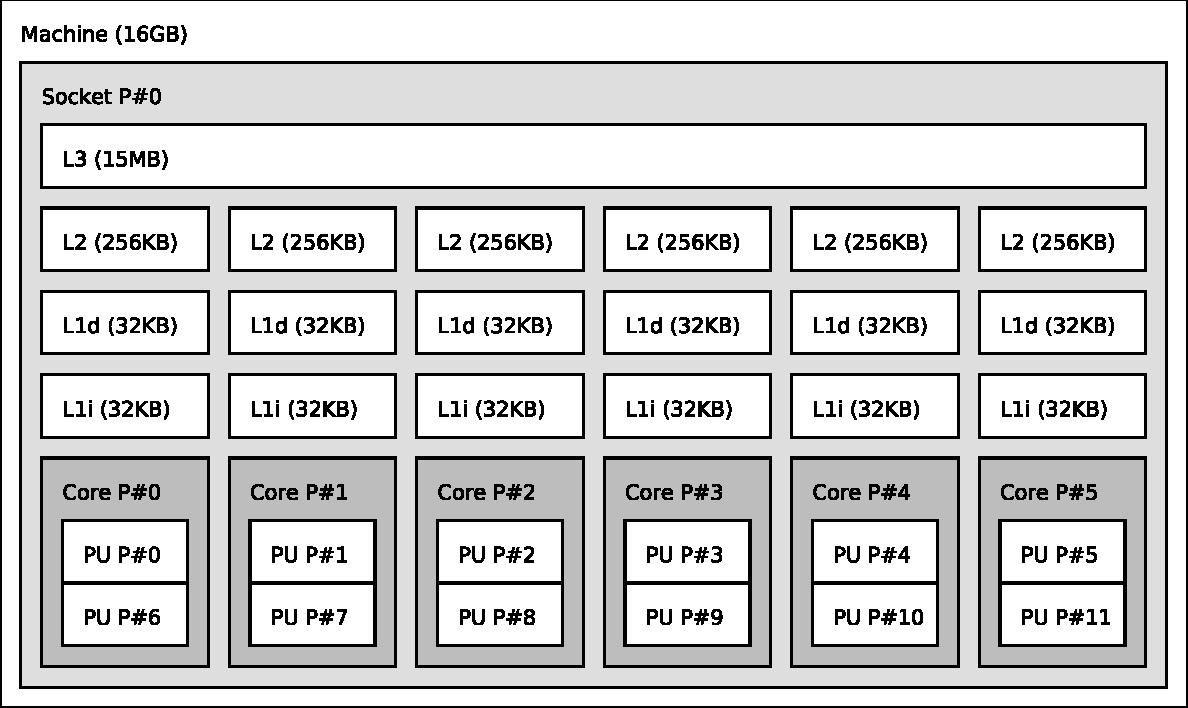
\includegraphics[width=\textwidth]{img/topo.pdf}
	\caption{Jerarquía de memoria de la maquina de pruebas.}

	\label{topoMemoria}

\end{figure}

\section{Resultados}

Durante el desarrollo de la aplicación se probaron tres distintas
implementaciones. En la primera implementación, el framework ejecutaba las
distintas pilas de plugins en tareas separadas. En la segunda implementación el
framework fue modificado para que una sola tarea ejecutara todas las pilas de
plugins sobre un mismo fragmento. Para la tercera implementación se trabajo
sobre el mismo framework que la segunda, pero se unieron las pilas de búsquedas
de robots y la de búsqueda de pelota. Para comprobar cual de estas era la mas
efectiva se realizaron las pruebas con cada una de estas para la configuración
de 12 hilos de búsqueda y 12 particiones con el vídeo de 1280x720 píxeles de
resolución. La primera implementación proceso XX \emph{FPS}, la segunda XX
\emph{FPS} y la tercera XX \emph{FPS}. Como esta última fue la que produjo
resultados mas satisfactorios, sera sobre los resultados de esta que
trabajaremos a continuación.

En las figuras \ref{800fps} y \ref{1280fps} se muestran las cantidades de
\emph{FPS} alcanzados para un vídeo de 800x600 píxeles y 1280x720 píxeles
respectivamente, para distintas cantidades de threads de búsqueda y fragmentos.
El numero de threads de búsqueda indica la cantidad de threads que ejecutan las
tareas dinámicas. Adicionalmente el sistema ejecuta dos threads más para las
tareas estáticas, uno para la generación de cuadros y otro para la tarea de
generación de tareas dinámicas. En el caso de del vídeo de 800x600 píxeles se
llego a un máximo de 195 \emph{FPS} cuando se divide el cuadro en 15 fragmentos
y se utilizan 10 u 11 hilos de busqueda, mientras que para el vídeo de 1280x720
píxeles se alcanzo un máximo de 94 \emph{FPS} cuando se divide el cuadro en 21
fragmentos y se utilizan 10 u 11 cuadros de búsqueda.

\begin{figure}[!h]

	\includegraphics[width=\textwidth]{img/800x600_fps.pdf}
	\caption{}
	\label{800fps}

\end{figure}

\begin{figure}[!h]

	\includegraphics[width=\textwidth]{img/1280x720_fps.pdf}
	\caption{}
	\label{1280fps}

\end{figure}

En las figuras \ref{800fps} y \ref{1280fps} se pueden observar dos patrones que
ocurren en ambos vídeos. El primero es que si los cuadros se dividen en 7, 11,
17, 19 y 23 fragmentos, se produce una notable reducción en la cantidad de
cuadros por segundo con respecto a las divisiones adyacentes. El segundo patrón
que se puede observar es una reducción en la cantidad de cuadros por segundo
cuando la cantidad de fragmentos es reducida y la cantidad de hilos de búsqueda
alta.

Cuando se incrementan la cantidad de fragmentos aumenta el área compartida y por
lo tanto el área total que se procesa, al mismo, una mayor cantidad de
fragmentos permite aprovechar mejor el paralelismo. Si se divide el cuadro en un
número primo de fragmentos, el área total se incrementa de forma significativa
con respecto a los valores circundantes. En la figura \ref{primosArea} se
muestra la fluctuación del área para cada cantidad de particiones desde 1 hasta
100 para un vídeo de 1280x720 píxeles de resolución, resaltando el crecimiento
para valores primos y para los valores inmediatamente inferiores y superiores.
Como puede observarse, a partir de 7 fragmentos el área total se incrementa de
forma significativa cuando el número es primo con respecto a los valores
cercanos no primos. Esto lleva a que un cambio mínimo en las posibilidades de
aprovechar el paralelismo se vea acompañado por un gran incremento en el área a
procesar.

\begin{figure}[!h]

	\includegraphics[width=\textwidth]{img/primos_area.pdf}
	\caption{}
	\label{primosArea}

\end{figure}

Para comprobar como esta variación de volumen de datos afecta la cantidad de
cuadros por segundo procesados, se realizaron nuevas pruebas sobre el vídeo de
1280x720 píxeles de resolución, con 11 hilos de búsqueda y variando la cantidad
de fragmentos entre los números primos mayores a 24 y menores a 100, y sus
inmediatos superior e inferior. Los valores para números primos e inmediatos
inferiores a 24 fueron tomados de los experimentos anteriores. Los resultados
pueden ser observados en la figura \ref{primosFPS}.

\begin{figure}[!h]

	\includegraphics[width=\textwidth]{img/primos_fps.pdf}
	\caption{}
	\label{primosFPS}

\end{figure}

Como se puede observar en la figura, para una cantidad de fragmentos menor a 7,
el perjuicio por aumento en el área es menor que el beneficio aportado por el
incremento en el paralelismo. Si se observa la figura \ref{primosArea}, dividir
el cuadro en 7 fragmentos resulta en el primer incremento notable de área con
respecto tanto a un fragmento menos como un fragmento más. También se pueden
apreciar que los incrementos repentinos en el área total coinciden con
disminuciones repentinas en los cuadros por segundo procesados.

El segundo patrón observado es que cuando la cantidad de fragmentos es baja y la
cantidad de hilos de búsqueda alta, el sistema tiene menor desempeño que
utilizar una menor cantidad de hilos de búsqueda pero una mayor cantidad de
fragmentos. Si la cantidad de fragmentos es menor que la cantidad de hilos de
búsqueda, siempre se estarán procesando por lo menos dos cuadros, y si la
cantidad de fragmentos uno menor que la mitad de los hilos de búsqueda, entonces
siempre se estarán procesando por lo menos tres cuadros. Esto tiene como efecto
que los cuadros compitan por la cache y reduce las posibilidades de que los
fragmentos entren completamente en las caches de nivel mas bajo. Por esto se
propuso la hipótesis de que el retardo se produce debido a un aumento en los
fallos de cache.

Para comprobar que la hipótesis es correcta se ejecuto el programa procesando el
vídeo de 1280x720 píxeles de resolución, donde cada curva muestra los resultados
de dividir la imagen en 1, 2, 6 o 12 fragmentos, variando la cantidad de hilos
de búsqueda de 1 a 11 y midiendo los fallos de cache. Para obtener los fallos de
cache se utilizo la herramienta \emph{perf}. Esta es una aplicación que permite
acceder a los contadores de hardware del procesador, lo que provee datos muy
precisos y sin overhead que modifique los datos. Los resultados pueden ser
observados en la figura \ref{cacheFallos}.

\begin{figure}[!h]

	\includegraphics[width=\textwidth]{img/cache_fallos.pdf}
	\caption{}
	\label{cacheFallos}

\end{figure}

Si se observa detenidamente cada curva de la figura, se pueden distinguir una
etapa de crecimiento acelerado, seguido de una etapa de crecimiento mas gradual.
En los casos de 1 y 2 fragmentos, el cambio es pronunciado, y se puede verificar
en la figura \ref{1280fps} que es justamente bajo esta configuración donde, dado
ese numero de fragmentos, agregar un hilo de búsqueda más reduce la cantidad de
cuadros procesados.

Finalmente, en las figuras \ref{800turnArround} y \ref{1280turnArround} se
pueden observar los tiempos máximos de espera de procesamiento de los cuadros,
para los vídeos de 800x600 y 1280x720 píxeles de resolución limitando los
cuadros por segundo generados al máximo encontrado en los experimentos
anteriores.

\begin{figure}[!h]

	\includegraphics[width=\textwidth]{img/800x600_turnArround.pdf}
	\caption{}
	\label{800turnArround}

\end{figure}


\begin{figure}[!h]

	\includegraphics[width=\textwidth]{img/1280x720_turnArround.pdf}
	\caption{}
	\label{1280turnArround}

\end{figure}

Estos dos últimas figuras nos permiten apreciar que no siempre una mayor
cantidad de cuadros por segundos procesados implicara el tiempo de retardo
mínimo. Dependiendo de si se desea minimizar el retardo de procesamiento de los
cuadros, maximizar la cantidad de cuadros procesados, o encontrar un balance
especifico, se deberá elegir una cantidad de fragmentos y procesadores
apropiada. Por ejemplo, en el caso del vídeo de 1280x720 píxeles de resolución,
dividir la imagen en 21 fragmentos y utilizar 11 permite procesar 94 cuadros por
segundo en el equipo de prueba, sin embargo el retardo es de $0.09$ segundos. Si
el cuadro se divide en 15 fragmentos y se utilizan 11 hilos de búsqueda, la
cantidad de cuadros por segundo procesados se cae a 90, pero el retardo se
reduce a $0.05$ segundos.
